\documentclass[12pt]{exam}
\usepackage{amsmath}
\usepackage{amssymb}
\usepackage{amsthm}
\usepackage{tikz}
\usepackage{mathtools}
\usepackage{graphicx}
\usepackage{wrapfig}

\usepackage{bm} %bold symbols
\usepackage{hyperref} %add links

%%%%%%%%%%%%%%%%%%%%%%%%%
% 	Define vars here 	%
%%%%%%%%%%%%%%%%%%%%%%%%%

\def\hwName{Homework Set 4: §14.1 – 14.5}
\author{Zhengyu James Pan} %use like \@author
\def\email{jzpan@umich.edu}
\makeatletter

\begin{document}
%Header
\pagestyle{head}
\firstpageheader{}{}{}
\header{MATH 215}{\hwName}{\thepage}

%Solution formatting
\printanswers
\unframedsolutions

%Top matter
{\parindent0in
\begin{center}
	\bf MATH 215 FALL 2023\\
	\bf \hwName \\
	\@author\ (\href{mailto:\email}{\email})
\end{center}
}

\begin{questions}
%1
\question Do Exercise 32 of §14.1 of Stewart’s Multivariable Calculus.
%\clearpage
%2
\question Do Exercises 61-66 of §14.1 of Stewart’s Multivariable Calculus.
%\clearpage
%3
\question Do Exercise 6 of §14.3 of Stewart’s Multivariable Calculus.
%\clearpage
%4
\question 
	\begin{parts}
		\part Suppose $g(x, y) = \sqrt{9 - 9x^2 - y^2}$. Draw a contour map for g and then sketch the graph of $g$.
		\part Draw a contour map of the function $m(x, y) = \frac{x}{(x2 + 3y2)}$, showing and labelling several level curves.
		curves.
	\end{parts}
%5
\question 
	\begin{parts}
		\part Use a linear approximation to estimate $(0.99)3 + (2.01)3 - 6(0.99)(2.01)$.
		\part Let $f(x, y) = xe^{y^2} - ye^{x^2}$ and find the equation for the tangent plane to the graph of $f$ at (1, 2).
		\part What point on the surface $z = x^2 - y^2$ has a tangent plane parallel to the plane found in the previous part?
	\end{parts}
%6
\question The wave heights h in the open sea depend on the speed $v$ of the wind and the length of time $t$ that the wind has been blowing at that speed. Values of the function $h = f (v, t)$ are recorded in feet in the following table:
	\begin{center}
		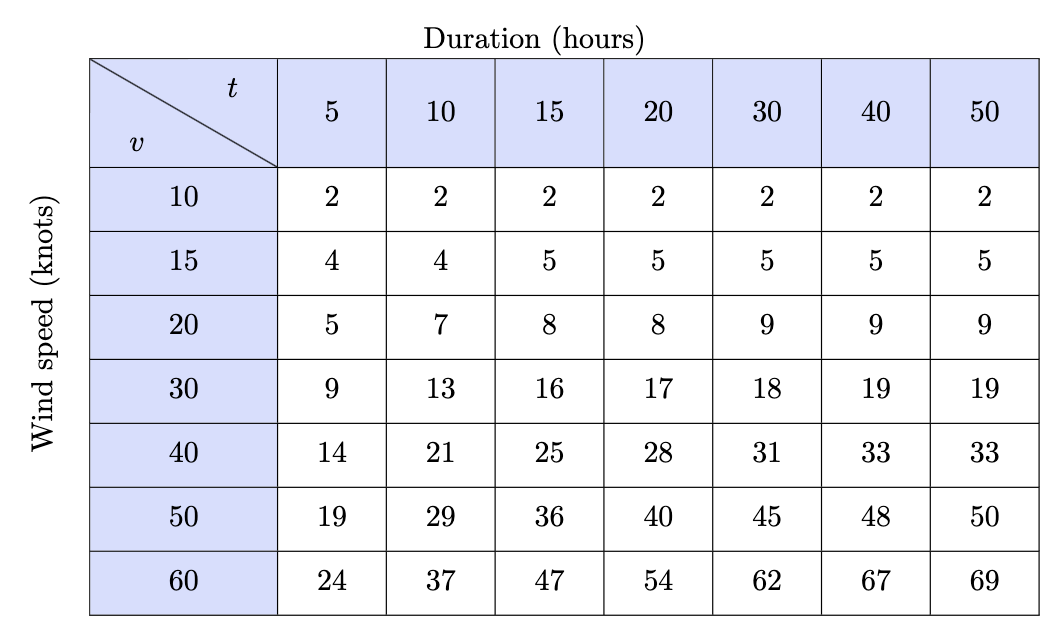
\includegraphics[scale = 0.8]{images/04-table.png}
	\end{center}
	\begin{parts}
		\part What are the meanings of the partial derivatives $\frac{\delta h}{\delta v}$ and $\frac{\delta h}{\delta t}$?
		\part Estimate the values of $f_v (40, 15)$ and $f_t(40, 15)$. What are the practical interpretations of these values?
		\part Estimate the values of $f_{vv} (30, 20), f_{tt}(30, 20), f_{vt}(30, 20)$, and $f_{tv} (30, 20)$. Are your answers for $f_{tv}$
		the same as for $f_{vt}$? Should they be? Explain. Hint: This problem might be trickier than it looks.
	\end{parts}
%7
\question Determine which of the following functions is a solution to Laplace’s equation uxx + uyy = 0:
	\begin{parts}
		\part 
	\end{parts}

%8
\question 
%9
\question Consider the function 
	\begin{equation*}
		f(x,y) = 
		\begin{cases}
			\frac{x^3y-xy^3}{x^2+y^2} & \text{ if } (x,y) \neq (0, 0) \\
			0 &\text{ if } (x,y) \neq (0, 0)
		\end{cases}
	\end{equation*}
	\begin{parts}
		\part Based on the plot of the level curves above, does it appear that $f$ is continuous at (0, 0)? Explain.
			\begin{solution}
				No, it does not appear to be continuous because the contour lines are not continued at (0, 0). Thus, it looks like an open point or sudden jump in the function.
			\end{solution}
		\part Find $f_x(x, y)$ and $f_y (x, y)$ when $(x, y) \neq (0, 0)$.
			\begin{solution}
				\begin{align*}
					f_x(x,y) &= \frac{(x^2+y^2)(3x^2y-y^3)-(x^3y-xy^3)(2x)}{(x^2+y^2)^2} \\
					&= \frac{3 x^4 y - x^2 y^3 + 3 x^2 y^3 - y^5 - 2 x^4 y + 2x^2 y^3}{(x^2 + y^2)} \\
					&= \boxed{\frac{x^4y + 4x^2y^3 - y^5}{(x^2+y^2)^2}} \\\\
					f_y(x, y) &= \frac{(x^2+y^2)(x^3-3xy^2)-(x^3y-xy^3)(2y)}{(x^2+y^2)^2} \\
					&= \frac{x^5 - 3 x^3 y^2 + x^3 y^2 - 3 x y^4 - 2 x^3 y^2 + 2 x y^4}{(x^2+y^2)^2} \\
					&= \boxed{\frac{x^5 - 4 x^3 y^2 - x y^4}{(x^2+y^2)^2}}
					\tag*{\qed}
				\end{align*}
			\end{solution}
		\part Can you use your answers from the previous part to find $f_x(0, 0)$ and $f_y (0, 0)$? Explain.
			\begin{solution}
				Yes, since the piecewise $f(0, 0) = 0$ patches the hole in $f$, so we can take the derivative at (0, 0).
			\end{solution}
		\part Using the definition of the partial derivative, find $f_x(0, 0)\text{ and }f_y (0, 0)$.
			\begin{solution}
				\begin{align*}
					f_x (0, 0) &= \displaystyle\lim_{h\rightarrow0} \frac{f(0+h, 0) - f(0,0)}{h} \\
					&= \displaystyle\lim_{h\rightarrow0} \frac{\frac{(x+h)^3y-(x+h)y^3}{(x+h)^2+y^2} - f(0,0)}{h} \\
					&= \displaystyle\lim_{h\rightarrow0} \frac{\frac{0-0}{x^2+2hx+h^2} - 0}{h} \\
					&= \displaystyle\lim_{h\rightarrow0} \frac{\frac{0}{h^2}}{h} \\
					&= \boxed{0}\\\\
					f_y (0, 0) &= \displaystyle\lim_{h\rightarrow0} \frac{f(0,0+h) - f(0,0)}{h} \\
					&= \displaystyle\lim_{h\rightarrow0} \frac{\frac{x^3(y+h)-x(y+h)^3}{x^2+(y+h)^2} - 0}{h} \\
					&= \displaystyle\lim_{h\rightarrow0} \frac{\frac{0}{h^2} - 0}{h}\\ 
					&= \boxed{0}
				\end{align*}
			\end{solution}
		\part Using the definition of the partial derivative, show $f_{xy} (0, 0) = -1\text{ and }f_{yx}(0, 0) = 1$.
		\part Does the result from the previous part contradiction Clairaut's Theorem? Justify you reasoning.
		Hint: Contour plots, possible generated using something similar to how we plotted a contour from
		MatLab above, might be a way to help bolster your explanation.
	\end{parts}
\end{questions}

\end{document}